% LaTeX Article Template - customizing page format
%
% LaTeX document uses 10-point fonts by default.  To use
% 11-point or 12-point fonts, use \documentclass[11pt]{article}
% or \documentclass[12pt]{article}.
\documentclass{article}

% Set left margin - The default is 1 inch, so the following 
% command sets a 1.25-inch left margin.
\setlength{\oddsidemargin}{0.25in}

% Set width of the text - What is left will be the right margin.
% In this case, right margin is 8.5in - 1.25in - 6in = 1.25in.
\setlength{\textwidth}{6in}

% Set top margin - The default is 1 inch, so the following 
% command sets a 0.75-inch top margin.
\setlength{\topmargin}{-0.25in}

% Set height of the text - What is left will be the bottom margin.
% In this case, bottom margin is 11in - 0.75in - 9.5in = 0.75in
\setlength{\textheight}{8in}
\usepackage{fancyhdr}
\usepackage{float}
\usepackage{mathtools}
\usepackage{amsmath}
\usepackage{amssymb}
\usepackage{graphicx}
\usepackage{float}
\graphicspath{ {./} }
\setlength{\parskip}{5pt} 
\pagestyle{fancyplain}
% Set the beginning of a LaTeX document
\begin{document}

\lhead{Drew Remmenga MATH 408}
\rhead{Project \#2}
%\lhead{Independent Study}
%\rhead{R Lab}

\begin{enumerate}

\item 
The function:
\begin{equation*}
\begin{split}
f(t,u) = u^{2}e^{-t^{2}}sin(t)
\end{split}
\end{equation*}
is Lipschitz continous in $u$ on:
\begin{equation*}
\begin{split}
 \mathcal{D} =\{(t,u): t\in \mathbb{R}, u \in [0,2]\}
\end{split}
\end{equation*}
if 
\begin{equation*}
\begin{split}
\exists L \in \mathbb{R_{+}} : \left|f(t,u) -f(t,u^{*}) \right| & \leq L \left| u - u^{*} \right| \\
\left|  u^{2}e^{-t^{2}}sin(t) - u^{*2}e^{-t^{2}}sin(t)  \right|  &\leq L \left| u - u^{*} \right| \\
\left|  u^{2}- u^{*2}  \right| \left|e^{-t^{2}}sin(t)\right|  &\leq L \left| u - u^{*} \right| \\
\left|  u- u^{*}  \right| \left|u+u^{*}\right| \left|e^{-t^{2}}sin(t)\right|  &\leq L \left| u - u^{*} \right| \\
\end{split}
\end{equation*}
Since $f(t,u)$ is differentiable with respect to $u$ and bounded in $\mathcal{D}$ then we can set the Lipschitz constant:
\begin{equation*}
\begin{split}
L &= \max_{(t,u) \in \mathcal{D}} \left| f_{u}(t,u) \right| \\
& =  \max_{(t,u) \in \mathcal{D}} \left| 2ue^{-t^{2}}sin(t) \right| \\
&\approx 4*.397 \\
& \approx 1.588 \\
\end{split}
\end{equation*}
\item
\begin{enumerate}
\item
Since $f(u)$ is differentible at all points $u \in \mathbb{R}$, $f(u)$ is Lipshitz at every point $u \in \mathbb{R}$.
With L $\leq$ 2.
\item
Take Dirchlet's 'jagged' discontinuous function which is continuous nowhere and is differentiable nowhere but is nonetheless bounded by 1.
\end{enumerate}
\item
\begin{equation*}
\begin{split}
f  &=
\begin{bmatrix}
u_{2} \\
-\frac{u_{1}}{(u_{1}^{2}+u_{3}^{2})^{3/2}} \\
u_{4}  \\
-\frac{u_{3}}{(u_{1}^{2}+u_{3}^{2})^{3/2}}
\end{bmatrix} \\
J(f) &= \begin{bmatrix}
0 & 1 & 0 & 0 \\
\frac{-2u_{1}^{2}+u_{3}^{2}}{(u_{1}^{2}+u_{3}^{2})^{5/2}} & 0 & \frac{-3u_{1}u_{3}}{(u_{1}^{2}+u_{3}^{2})^{5/2}} & 0 \\
0 & 0 & 0 & 1 \\
 \frac{-3u_{1}u_{3}}{(u_{1}^{2}+u_{3}^{2})^{5/2}} & 0 & \frac{-2u_{3}^{2}+u_{1}^{2}}{(u_{1}^{2}+u_{3}^{2})^{5/2}} & 0 \\
\end{bmatrix} \\
\end{split}
\end{equation*}
\begin{equation*}
\begin{split}
\left|\left| A\right|\right|_{F} & = \sqrt{\sum_{i}\sum_{j} \left| A_{ij} \right |^{2} } \\
\left|\left| A\right|\right|_{F} & = \sqrt{ 1^{2} + (\frac{-2u_{1}^{2}+u_{3}^{2}}{(u_{1}^{2}+u_{3}^{2})^{5/2}})^{2}+(\frac{3u_{1}u_{3}}{(u_{1}^{2}+u_{3}^{2})^{5/2}})^{2}+1^{2} +( \frac{3u_{1}u_{3}}{(u_{1}^{2}+u_{3}^{2})^{5/2}})^{2}+(\frac{-2u_{3}^{2}+u_{1}^{2}}{(u_{1}^{2}+u_{3}^{2})^{5/2}})^{2}}\\
\left|\left| A\right|\right|_{F} & = \sqrt{ 2 + \frac{4u_{1}^{4}+u_{3}^{4}-4u_{1}^{2}u_{3}^{2}}{(u_{1}^{2}+u_{3}^{2})^{5}}+\frac{18u_{1}^{2}u_{3}^{2}}{(u_{1}^{2}+u_{3}^{2})^{5}} +\frac{4u_{3}^{4}+u_{1}^{4}-4u_{3}^{2}u_{1}^{2}}{(u_{1}^{2}+u_{3}^{2})^{5}}}\\
\left|\left| A\right|\right|_{F} & = \sqrt{ 2 + \frac{5u_{3}^{4}+5u_{1}^{4}+10u_{3}^{2}u_{1}^{2}}{(u_{1}^{2}+u_{3}^{2})^{5}}}\\
\left|\left| A\right|\right|_{F} & = \sqrt{ 2 + \frac{5}{(u_{1}^{2}+u_{3}^{2})^{3}}}\\
(\left|\left| A\right|\right|_{F})^{2} & = 2 + \frac{5}{(u_{1}^{2}+u_{3}^{2})^{3}}\\
(\left|\left| A\right|\right|_{F})^{2}-2 & = \frac{5}{(u_{1}^{2}+u_{3}^{2})^{3}}\\
(u_{1}^{2}+u_{3}^{2})^{3} & = \frac{5}{(\left|\left| A\right|\right|_{F})^{2}-2}\\
\end{split}
\end{equation*}
\begin{equation*}
\begin{split}
\mathcal{D} := \{u: 1/4 \leq u_{1}^{2} + u_{3}^{2} \}
\end{split}
\end{equation*}
Apply this domain and we achieve an upper bound on $(\left|\left| A\right|\right|_{F})^{2}$
\begin{equation*}
\begin{split}
(\frac{1}{4})^{3} & \leq \frac{5}{(\left|\left| A\right|\right|_{F})^{2}-2}\\
(\left|\left| A\right|\right|_{F})^{2} &\leq 322
\end{split}
\end{equation*}
And is therefore Lipschitz.
\item
\begin{enumerate}
\item
\item
1.2830
		\begin{figure}[H]
		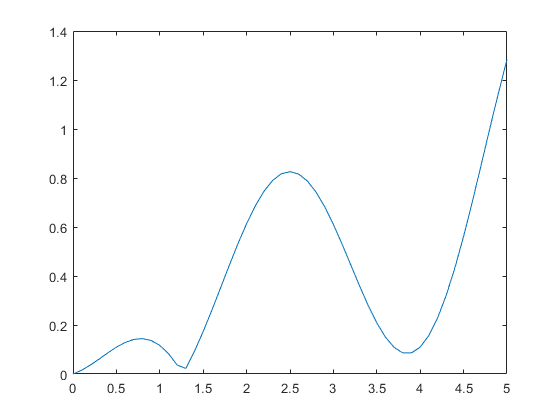
\includegraphics[scale=.5]{figure1.png}
		\end{figure}
\item
0.0149
		\begin{figure}[H]
		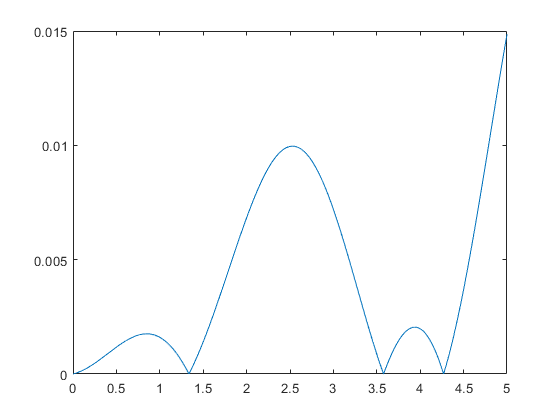
\includegraphics[scale=.5]{figure2.png}
		\end{figure}
\end{enumerate}
\item
\begin{enumerate}
\item
\item
.6563
		\begin{figure}[H]
		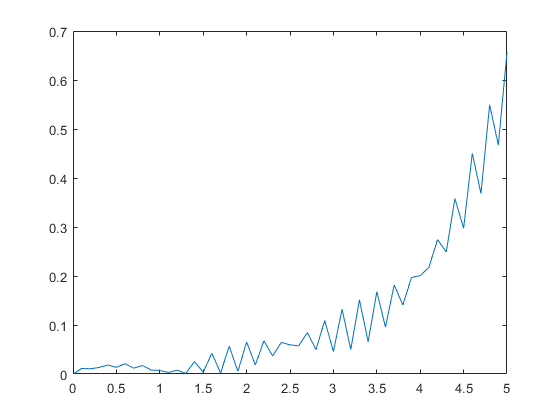
\includegraphics[scale=.5]{figure3.png}
		\end{figure}
\item
6.6262E-05 \\
		\begin{figure}[H]
		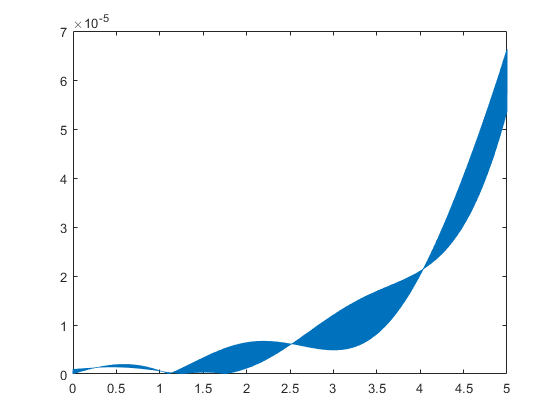
\includegraphics[scale=.5]{figure4.png}
		\end{figure}
\newpage
\end{enumerate}
\item
\begin{enumerate}
\item 
Backwards Euler
		\begin{figure}[H]
		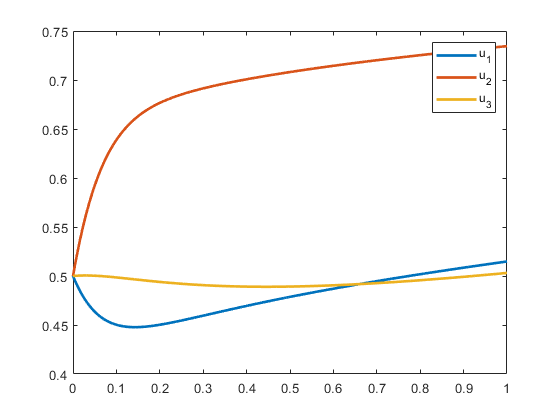
\includegraphics[scale=.5]{figure5.png}
		\end{figure}
\item
Leapfrog
		\begin{figure}[H]
		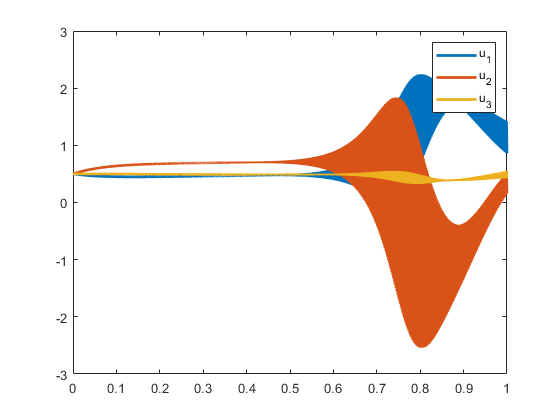
\includegraphics[scale=.5]{figure6.png}
		\end{figure}
\item
Leapfrog with smaller k
		\begin{figure}[H]
		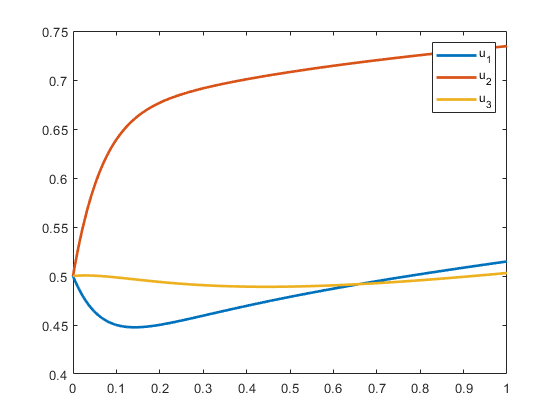
\includegraphics[scale=.5]{figure7.png}
		\end{figure}
\end{enumerate}
\end{enumerate}



\end{document}
